\chapter{ECM using Edwards curves}
\label{cha:ECMedwardsCurves}
This chapter serves as documentation for the implementation of ECM using Edwards curves the author made in connection with this thesis. We describe which techniques and speed ups we use. We also include a section of experiments/statistics that should provide an overview of the efficiency of the implementation. In the following the program will be refered to as \textit{EECM\_Torben}.

Generally any implementation of ECM that needs to be fast are essentially faced with the two following algorithmic challenges: Fast modular arithmetic and efficient curve operations. Efficient modular arithmetic will be provided by the \textit{BigInteger library} in Java and is therefore not a class implemented by the author. This is discussed in section \ref{sec:modularArithmetic}. Efficient curve operations is provided by (as you may have guessed) arithmetic on Edwards curves. How Edwards curves relate to the elliptic curve factorization method is discussed in \ref{sec:usingEDC}.

EECM\_Torben has the same general structure as algorithm \ref{alg:basicECM} but with some major differences.
\begin{itemize}
\item EECM\_Torben use Edwards curves instead of Weierstrass curves, and therefore instead of picking a curve $E_{W,a,b}(\Z/n\Z)$ we pick an Edwards curve $E_{E,d}$ and calculate over $\Z/n\Z$. 
\item When we have computed $[s]P$ we check the gcd between the $x$-coordinate and $n$. This is because the neutral element on the Edwards curve is $(0,1)$ (in projective $[0,1,1]$). At a first glance the addition formula in \ref{sec:effAddandAna} this seems to allow a factor of $n$ not to accumulate in the $x$-coordinate i.e. if one time during the calculation of $[s]P$ we find a factor of $n$ it is not clear that this factor remain present in the $x$-coordinate. But by inspecting the source code of EECM\_Torben one sees that factors indeed do accumulate, because we use the $x$-coordinate from the newly computed point as $x_2$ in the next iteration (see also algorithm \ref{alg:naf}). In the ordinary ECM algorithm one would check the $z$-coordinate when using projective Weierstrass coordinates. 
\item We use a second stage method to improve the probability of finding a factor. This implementation is discussed in section \ref{sec:implSecondStage}.
\item The calculation of $[s]P$ is done using a NAF representation of the primes. This is discussed in section \ref{sec:SSM}.
\item We do not check for $\gcd(6,n)$ and $n$ not being a perfect power. In practice EECM\_Torben find primes in $n$ whether or not it is a perfect power and since checking for $n$ being a perfect power is not extremely cheap we neglect this. Instead of checking the $\gcd$ between 6 and $n$ we instead do a trial division for all primes from 2 to 1000. these primes has been hard coded into EECM\_Torben and it is therefore really fast to do this check and is much more efficient than only trying to find a factor of 2 or 3 in $n$. Actually the bound 1000 may be varied depending of $n$ but it all comes down to how much time one want to spend doing trial division versus the time it takes to execute the rest of the algorithm. 
\end{itemize}

\section{Using Edwards curves}\label{sec:usingEDC}
There are obvious improvements from using Edwards curves. In \ref{sec:effAddandAna} we saw that arithmetic on Edwards curves is more efficient than doing arithmetic on Weierstrass curves and actually the formulas is some of the most efficient known. Also the reduced curve order is certain to be divisible by 4 because of theorem \ref{thm:pointoforderfour}. Heuristically this give a better chance of being smooth.

We also expect the approximate same complexity as the original ECM presented and analysed in chapter 2. This is because, reducing an Edwards curve, say $E_{E,d}$, over a positive integer $n$ with a prime $p$ dividing $n$ would give an ordinary Edwards curve. From remark \ref{rem:commentsProof} that if EECM\_Torben hit a point with a $x$-coordinate that is divisible by $p$ then it is probably the neutral element for the reduced Edwards curve by $p$. Theorem \ref{thm:EdCcorrespondEC} shows that the calculations that were done on the reduced Edwards curve corresponds to an birationally equivalent elliptic curve and that we from the reduced Edwards curve has hit the neutral element on the corresponding elliptic curve. Using the same considerations that we did in section \ref{sec:ECMcomplextiy} we see that the complexity should be unchanged. 

\section{Stage two}\label{sec:implSecondStage}
Stage 2 in EECM\_Torben is implemented as described in section \ref{sec:2StageECM} (using the last version). The implementation is called the standard continuation, but is implemented with some speed up tricks. 

In places where we need to add the same point to another a lot of times we normalize the point. This require 1\textbf{I}+2\textbf{M} but if e.g. $\textbf{I}/\textbf{M}=150$ we still save multiplications as long a we have to add the given point over approximately 150 times because a mixed addition is 1\textbf{M} cheaper than a dedicated addition. 

We also store multiples of 2 of the point $Q=\left[ \prod_{p_i^{a_i}\leq B_1}p_i^{a_i}\right] P$ up to some limit. This limit actually do not need to be very large! We do a little analysis. We need the precomputed points to calculate $[p_{i+1}-p_i]Q$ i.e. we need to pre compute $[2s]Q$ up to the biggest prime gap for primes below $B_2$. If $g_n=p_{n+1}-p_n$ denotes the prime gap between the $n$th and $(n+1)th$ prime then a maximal prime gap is a gap $g_n$ such that $g_n>g_m$ for all $m<n$. The distribution of the length of prime gaps is not that well understood, but there exists numerical results of maximal prime gaps for huge numbers (far greater than we need). On \url{http://www.trnicely.net/gaps/gaplist.html} Thomas Nicely host list of prime gaps including the maximal ones (in the lists these are indicated by an asterix mark). Since the magnitude of primes in EECM\_Torben is bounded to approximately 1.4 billion due to memory requirements, we do not need many multiples of 2 in our second stage. If one looks in Nicely's table one see that the maximal prime gap below 1.4 billion is 320 and since we only need multiples of 2 we need at most 160 precomputed points. This saves foremost a lot compared to computing e.g. $\frac{B_2}{2}$ multiples (which would be the naive choice) but memory requirements is also greatly reduced. 

There exists several improvements to the 2. stage. We give a high level description of some of these. One approach is: Take two integers $\tau$ and $\sigma$ and compute $[\tau] Q+[\sigma] Q$ where $Q$ is the point after the first stage. Set $[\tau]Q=(x_\tau,y_\tau)$ and $[\sigma]Q=(x_\sigma,y_\sigma)$. If $[\tau] Q+[\sigma] Q=\infi \mod p$ then $x_\tau \equiv x_\sigma \mod p$ and $\gcd(x_\tau-x_\sigma,n)>1$. The way $\tau$ and $\sigma$ is picked is how different continuations of this form differ. The birthday paradox form is to pick $\sigma\in T$ and $\tau\in S$ in two set $T,S\subset\N$. $T$ and $S$ are either picked out random or as geometric progressions. One then hope that all combinations $\tau+\sigma$ hits all primes in $[B_1,B_2]$. In addition one might hit larger primes. This approach may be optimized using fast polynomial arithmetic. A popular choice is to use a Fast Fourier Transformation. An extension of this kind is called a FFT extension. The polynomial arithmetic is applied, in different ways to obtain $\prod_{\tau\in S}\prod_{\sigma\in T}(x_\sigma-x_\tau)\mod n$ in a fast way. For more 2. stage continuations consult \cite{ZimmermannD06}.

\section{Modular arithmetic}\label{sec:modularArithmetic}
As mentioned, the modular arithmetic is provided by the BigInteger library from Java's standard library. There is two main reason for choosing this option. The first is while implementing a new big number library is doable then since the BigInteger library has been developed trough several years, creating a library that is faster must be considered a low probability event and something which would take a lot of time. The other reason is that it is not the scope of this thesis to develop a new big number library. We do not claim that a development of an efficient dedicated ring library is not worth the effort. It will with out doubt speed up computations because the BigInteger library we use is a big number library where modular arithmetic has been added subsequently. 

A reference to the methods used from the BigInteger library inside EECM\_Torben is \url{http://docs.oracle.com/javase/6/docs/api/java/math/BigInteger.html}

\section{Single-scalar multiplication}\label{sec:SSM}
The most time consuming operation in EECM\_Torben is the calculation of $\left[\prod_{p^{\alpha_i}\leq B_1} p^{\alpha_i}\right]P$ also called a single-scalar multiplication, see algorithm \ref{alg:basicECM}. For this to be fast we need efficient formulas for doubling and addition/subtraction on the Edwards curve and a good strategy for computing the point. We do not compute the product $\prod_{p^{\alpha_i}\leq B_1} p^{\alpha_i}$ and then calculate the point. Instead we do one prime at a time. First we discuss the arithmetic.

We saw in chapter \ref{cha:edwardsCurves} that the addition law is complete when $d$ is a non square. This is, as mentioned, a really good property if one want to use Edwards curves in cryptography or simplify code. But in this thesis we do not go for simplification, we go for speed. Since doubling on Edwards curves is faster than ordinary addition, we will not use the property of completeness. Instead we actually neglect the possibility that a non defined addition/doubling could occur; when $n$ is very large the probability that $dx_1x_2y_1y_2=\pm 1$ is very little. Below is shown register allocations of how we compute in EECM\_Torben using the formulas discussed in \ref{sec:effAddandAna}. The formulas are implemented in the class \textit{Edward}.

\textbf{Register allocations.} In the following $r_1$, $r_2$ and $r_3$ contains $x_1$, $y_1$ and $z_1$ respectively. $r_4$, $r_5$ and $r_6$ likewise contains $x_2$, $y_2$ and $z_2$. $r_7$ and $r_8$ are temporary registers.  

Addition $[x_1,y_1,z_1]+[x_2,y_2,z_2]$ (from left to right):
\begin{align*}
&r_3\leftarrow r_3\cdot r_6,\quad r_7\leftarrow r_1+r_2,\quad r_8\leftarrow r_4+r_5,\quad r_1 \leftarrow r_1\cdot r_4,\quad r_2\leftarrow r_2\cdot r_5,\quad r_7 \leftarrow r_7\cdot r_8 \\
&r_7 \leftarrow r_7-r_1, \quad r_7 \leftarrow r_7-r_2, \quad r_7 \leftarrow r_7\cdot r_3,\quad r_8 \leftarrow r_1\cdot r_2,\quad r_8\leftarrow d\cdot r_8,\quad r_2\leftarrow r_2-r_1,\\
&r_2 \leftarrow r_2\cdot r_3,\quad r_3\leftarrow r_3^2,\quad r_1\leftarrow r_3-r_8,\quad r_3\leftarrow r_3+r_8,\quad r_2\leftarrow r_2\cdot r_3,\quad r_3\leftarrow r_3\cdot r_1, \\
&r_1\leftarrow r_1\cdot r_7.
\end{align*}

Doubling $2[x_1,y_1,z_1]$ (from left to right):
\begin{align*}
&r_4\leftarrow r_1+r_2,\quad r_1\leftarrow r_1^2,\quad r_2\leftarrow r_2^2,\quad r_3\leftarrow r_3^2,\quad r_4\leftarrow r_4^2,\quad r_3\leftarrow r_3+r_3,\quad r_5\leftarrow r_1+r_2, \\
&r_2\leftarrow r_1-r_2,\quad r_4\leftarrow r_4-r_5,\quad r_3\leftarrow r_5-r_3,\quad r_1\leftarrow r_3\cdot r_4, \quad r_3\leftarrow r_3\cdot r_5,\quad r_2\leftarrow r_2\cdot r_5.
\end{align*}

Mixed addition does not need the first computation in the addition allocations. Subtraction is done by first calculating the additive inverse and then call addition. This means that subtraction cost a very tiny bit more than addition.

\textbf{NAF.} Here we describe the strategy used to compute $\left[\prod_{p^{\alpha_i}\leq B_1} p^{\alpha_i}\right]P$ in particular we describe the addition chain being used. Say $A$ is an array containing the primes from 2 to $B_1$. We want to optimize the following computation where $P$ is some point
\begin{algorithm}
\caption{Basic calculation of $\left[\prod_{p^{\alpha_i}\leq B_1} p^{\alpha_i}\right]P$}
\begin{algorithmic}
\label{alg:optimize}
\FOR{$i=0\to \vert A\vert-1$}
\STATE $p=A[i]$
\STATE $j=1$
\WHILE{$p^j\leq B_1$}
\STATE $P=[p]P$
\STATE $j=j+1$
\ENDWHILE
\ENDFOR
\end{algorithmic}
\end{algorithm}
First idea is to use a binary ladder. If a number $\beta$ is written in its binary decomposition $\beta = \sum_{i} a_i2^i$ with $a_i\in \{1,0\}$, on average $\frac{1}{2}$ of the numbers $a_i$ is zero. We are not satisfied with that. Instead we use a NAF (Non-adjacent form) representation introduced by Reitwieser in \cite{reitwiesner:binary}. We use the property that any number $\beta$ may be written as $\beta =\sum_i b_i2^i$ with $b_i\in\{1,0,-1\}$ and the additional property $b_ib_{i+1}=0$. This may add one additional bit to the representation compared to the binary decomposition but instead on average $\frac{1}{3}$ of the $b_i$'s are 0 (proved by Morain and Olivos in \cite{Morain&Olivos:1990}). Generally the NAF representation is a unique signed-digit representation but in our representation we do not need a sign and hence the most significant bit is always 1. The two algorithms \ref{alg:computeNAF} and \ref{alg:naf} compute what we need in EECM\_Torben

\begin{algorithm}
\caption{Compute NAF representation}
\begin{algorithmic}
\label{alg:computeNAF}
\REQUIRE Positive integer $n$.
\ENSURE NAF representation $(n_0,n_1,\ldots,n_i)$ of $n$.
\STATE $j=0$
\WHILE{$n>0$}
\IF{$n$ odd}
\STATE $n_j=2-[n]_4$
\STATE $n = n-n_j$
\ELSE
\STATE $n_j=0$
\ENDIF
\STATE $n=\frac{n}{2}$
\STATE $j=j+1$
\ENDWHILE
\end{algorithmic}
\end{algorithm}
Notice that in algorithm \ref{alg:computeNAF} if $n$ is odd in some iteration of the while loop, we make $n$ divisible by 4. Hence when we divide out by two in the end of the while loop, The number remains even and therefore the next bit will be set to 0 forcing the condition $b_jb_{j+1}=0$. If $n$ is an $i$ bit number then its NAF representaion has either $i$ or $i+1$ bits. 

\begin{algorithm}
\caption{NAF calculation of $\left[\prod_{p^{\alpha_i}\leq B_1} p^{\alpha_i}\right]P$}
\begin{algorithmic}
\label{alg:naf}
\REQUIRE Point $P$ and a table of primes $Q$ from 1 to $B_1$. 
\ENSURE The single scalar multiplication $\left[\prod_{p^{\alpha_i}\leq B_1} p^{\alpha_i}\right]P$ 
\FOR{$i=0 \to \vert Q\vert-1$}
\STATE $j=1$
\STATE $p=Q[i]$
\WHILE{$p^j\leq B_1$}
\STATE Compute NAF of $p$; $(n_0,n_1,\ldots,n_l)$, using algorithm \ref{alg:computeNAF}
\STATE $\overline{P}=P$
\FOR{$s=l \to 1$}
\STATE $P.dup()$
\IF{$n_s=1$}
\STATE $P = P.add(\overline{P})$
\ENDIF
\IF {$n_s=-1$}
\STATE $P = P.sub(\overline{P})$
\ENDIF
\ENDFOR
\STATE $\overline{P}=P$
\STATE $j=j+1$
\ENDWHILE
\ENDFOR
\end{algorithmic}
\end{algorithm}

Compared to algorithm \ref{alg:optimize}, algorithm \ref{alg:naf} has several advantages. The number of additions is greatly reduced and we trade a lot of dedicated additions with doublings which is cheaper. 

There exists various other single-scalar multiplication schemes that can be deployed. Instead of using a window of 2 one could use a window of 4 or even greater. In \cite{cryptoeprint:2007:414} Bernstein et al. also discusses a double-base single-scalar multiplication with a basis $\{2,3\}$. Another method is to use a sliding window; compute point $[a]P$ where $a$ is a member of some basis e.g. $\{1,2,3,4,9\}$. This is also discussed in the paper by Bernstein et al.

\section{Bounds $B_1$ and $B_2$}
Bounds $B_1$ and $B_2$ are really the key if one wants to find a factor. In section \ref{sec:ECMcomplextiy} we saw that finding a factor, say $p$, of $n$ really depends on whether the curve order of the reduction with $p$ is $B_1-$power smooth or not. $B_1$ could be picked optimal if $p$ is known, but of course this knowledge will totally ruin the need for using ECM. Instead one must experiment with different values. In practice, what is done is that one value $B_1$ is run sufficiently many times without success for one to become convinced that a higher value is called for. One normally starts with a low $B_1$ value (In EECM\_Torben the default value for $B_1$ is 10000 and for $B_2$ its 100000) and maybe increase by a factor of 100, or double the value. The bound $B_2$ is also a debatable value. In \cite{pomeranceEt.al} (p. 343) it is suggested that when using a highly efficient second stage (such as a FFT extension) one should pick $B_2\approx 100 B_1$. In EECM\_Torben we use $B_2=10B1$ since we do not use the highly advanced speed ups discussed in \cite{pomeranceEt.al}. This also depends on your baby (your computer red.). The conventional wisdom is that stage 1 and stage 2 should take an approximate equal amount of time to process one curve. 

In \cite{SilvermanWagstaff:1993} Silverman and Wagstaff propose optimal values for $B_1$ and $B_2$ depending on the factor size one is searching for. That is, if we search for a factor size of 20 digits say, they suggest values for $B_1$ and $B_2$ that give a high probability of finding this factor. Paul Zimmermann has likewise computed optimal parameters for the bound $B_1$ and suggest the expected amount of curves which is needed with respect to the factor size one search for. This can be found here \url{http://www.loria.fr/~zimmerma/records/ecm/params.html}. It should be taken into account that these estimates are relatively old i.e. was made before the invention of more advanced second stage methods (e.g. the FFT 2. stage).

Considering the former discussion the author has made the bounds in EECM\_Torben configurable by the flags $-B1$ and $-B2$ e.g. if a user wants to change the bounds to $B_1=10^6$ and $B_2=10^7$ one input $-B1100000$ $-B21000000$. The program does not allow a $B_2$ value that is lower than $B_1$. Also a factor size flag has been added implementing Zimmermans scheme; accessed by the flag $-FS$ e.g. if one search for a factor of size, say 23 digit, then input option $-FS23$. Note that both inputting a factor size and bounds will make the program skip the factor size option. 

\section{Curve selection}
EECM\_Torben is using the following method for picking a suitable curve. Pick $x,y\underset{R}\in \Z/n\Z$ such that $\gcd(xy,n)=1$. Then we may set $(x^2+y^2-1)(x^2y^2)^{-1}=d$ and check if $d\neq 1$ (In practice we do not need to check for $d=0$). If one of these checks is false, then pick two new elements in $\Z/n\Z$. $(x,y)$ is now a point on the Edwards curve $E_{E,d}$ over $\Z/n\Z$. Below we discuss other (and possible more efficient) ways to do it. The theory behind is not discussed in this thesis and proof are omitted, but references are given. To specify the number of curves EECM\_Torben should maximally process input the option $-NC$.

In \cite{2011/BBLP-eecm} Bernstein et al. present two different parametrisations for Edwards curves (and one for the more general twisted Edwards curves); the Atkin-Morain construction and the Montgomery construction which are both well known constructions for ordinary elliptic curves, is translated to Edwards curves. The Atkin-Morain and Montgomery construction force torsion groups $\Z/2\Z\times \Z/8\Z$ and $\Z/12\Z$ respectively. Below we present the two different construction.
\begin{thm}
(Atkin-Morain on Edwards curves) Pick a point $(s,t)$ on $E_{W,-8,-32}(\Q)$ and define $\alpha=\left(\frac{t+25}{s-9}+1\right)^{-1}$, $\beta=2\alpha\frac{4\alpha+1}{8\alpha^2-1}$ and $d=\frac{2(2\beta-1)^2-1}{(2\beta-1)^4}$. Then $E_{E,d}$ has torsion group isomorphic to $\Z/2\Z\times \Z/8\Z$ and a point $(x,y)$ with $x=\frac{(2\beta-1)(4\beta-1)}{6\beta-5}$ and $y=\frac{(2\beta-1)(t^2+50t-2s^3+27s^2-104)}{(t+3s-2)(t+s+16)}$
\end{thm}
Finding points $(s,t)$ may be done by choosing $(s,t)=(12,40)$ and computing multiples. 
\begin{thm}
(Montgomery on Edwards curves) Pick a point $(s,t)$ on $E_{W,-12,0}(\Q)$ with $(s,t)\notin \{(0,0),(-2,\pm 4),(6,\pm 12)\}$. Define $d=\frac{-(s-2)^3(s+6)^3(s^2-12s-12)}{1024s^2t^2}$. Then $E_{E,d}$ has torsion group isomorphic to $\Z/12\Z$ and point $(x,y)$ with $x=\frac{8t(s^2+12)}{(s-2)(s+6)(s^2+12-12}$ and $y=\frac{-4s(s^2-12s-12)}{(s-2)(s+6)(s^2-12)}$
\end{thm}

\textbf{Hard coded curves}
In \cite{2011/BBLP-eecm} the authors went even further than ensuring large torsion groups. They constructed curves with small parameters, large torsion and positive rank which, heuristically, should give a speed up. These ``good curves'' can be found on \url{http://eecm.cr.yp.to/goodcurves.html}. This optimization has not been implemented in EECM\_Torben. 

\section{Prime generation}
We need a lot of primes for both stage 1 and 2. The number of primes is bounded by the stage 2 bound $B_2$. For finding these primes we use Erasthosthenes sieve. This works by first creating a list from 2 to $B_2$ (if $B_2$ is odd otherwise we only need up to $B_2-1$). Take the smallest number in the list; 2, and cross out all its multiples up to $B_2$. Continue by taking the next number in the list that has not been crossed (this will be 3) out and cross out all the multiples of this number up to $B_2$. Continue by taking the next number in the list that has not been crossed out (will be 5) and cross out all the multiples of this number up to $B_2$.... Continue until we reach $\sqrt{B_2}$. All numbers not crossed out are the primes up to  $B_2$. 

The implementation of Erathosthenes sieve is provided by the author. We use several speed ups e.g. To minimize the memory needed we only store odd numbers and we only check odd multiples of a prime. This sieving method is extremely fast; amortized using only $O(\log\log B_2)$ work per prime. The drawback is the memory requirement. We save a factor of 2 by only storing odd numbers but we are still in the need of $\frac{B_2}{2}$ space. It is not optimal but sufficient for our purpose. 

Some optimizations for the memory use and speed is: Use a segmented sieve where sieving is done in segments. This reduce the memory need for the sieving array to the size of the segment. One may consider Erasthosthenes sieves as a segmented sieve with just one segment. One way to obtain a significant speed up is to implement a wheel in which you skip multiples of 2, 3, 5,.. up to some limit. This may also reduce the memory requirements. 

\section{Additional comments}
On a machine with multiple cores (which modern machines normally has (or should have)) a significant speed up may be archived by distributing the work of an algorithm among the cores. ECM is particular easy to parallellize; One may run one (or more) curves on each core. In EECM\_Torben this is done by implementing the \textit{Runnable} interface. Although in Java you are not 100\% certain that all cores are used. The user may specify how many threads that should be used with the option $-NT$ (The number of threads running at the same time, not the total number of threads).   

\section{Experiments}\label{sec:experimentsEdward}
In this chapter we present performance tests for EECM\_Torben. The method used is the following: For a random $\beta$-bit prime we picked a random $200-\beta$-bit prime and multiplied these together to obtain a 200-bit number with two prime factors. For a particular $\beta$-bit prime a sample set of 500 numbers was created. It was then run with EECM\_Torben using the option $-FS\alpha$ where the factor size $\alpha$ with $\alpha \approx \frac{\beta}{3}$ factor 
We have measured: Time, number of curves, number of modular multiplications (multiplications and squaring) and the total number of modular operations. 

The following charts are average plots e.g. a run with the 15-bit sample set all times are added and divided with 500 to get the average time over the 500 samples. 
All output and sample set files may be downloaded by visiting \url{http://home.imf.au.dk/himsen/Cryptography.html}.
\begin{figure}[htp]
\centering
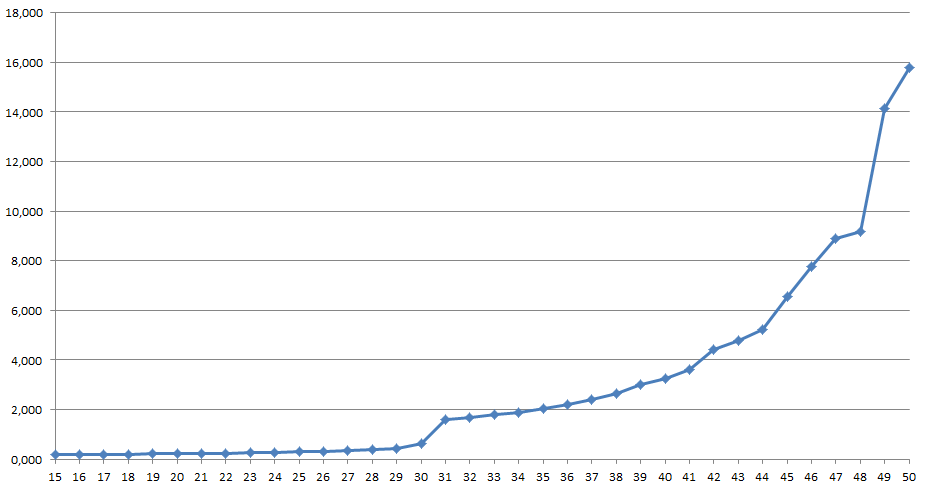
\includegraphics[scale=0.6]{stat_time.png}
\caption{Average time.}
\label{fig:dedicatedAddition}
\end{figure}
\begin{figure}[htp]
\centering
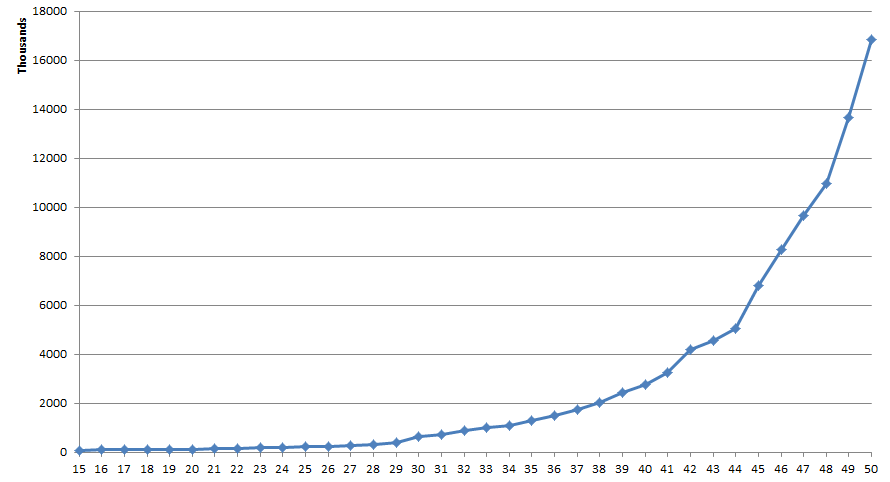
\includegraphics[scale=0.6]{stat_mult.png}
\caption{Average modular multiplications (multiplications+squarings).}
\label{fig:dedicatedAddition}
\end{figure}
\begin{figure}[htp]
\centering
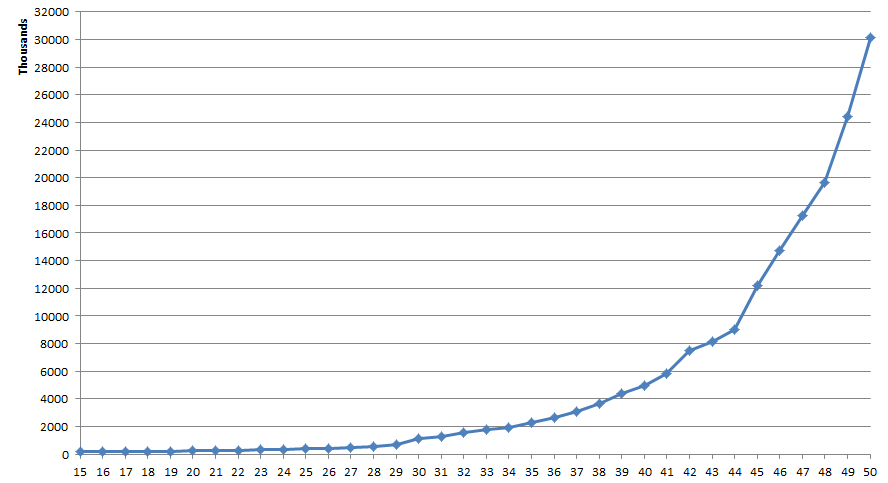
\includegraphics[scale=0.6]{stat_TotalMult.png}
\caption{Average total modular operations (multiplications+squarings+additions+inversions)}
\label{fig:dedicatedAddition}
\end{figure}
\begin{figure}[htp]
\centering
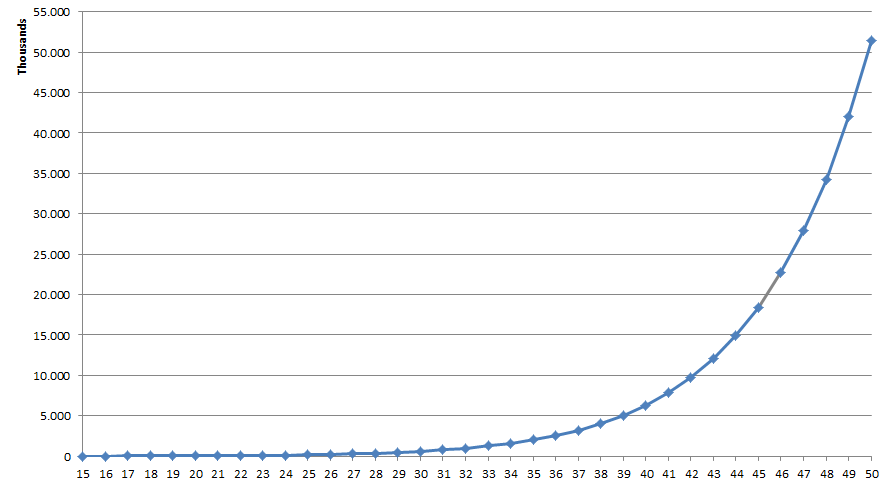
\includegraphics[scale=0.6]{stat_TotalMult_theory.png}
\caption{The theoretical total number of modular operations. For a $\beta$-bit factor
$8\cdot e^{\sqrt{2\ln(2^\beta)\ln(\ln(2^\beta))}}$ is plotted. See remark \ref{rem:theory}.} 
\label{fig:dedicatedAddition}
\end{figure}
\begin{figure}[htp]
\centering
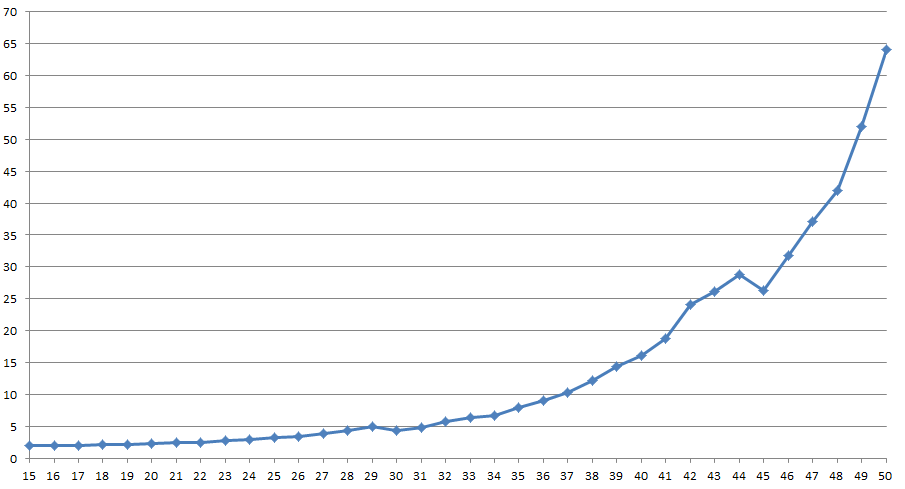
\includegraphics[scale=0.6]{stat_curves.png}
\caption{Average number of curves.}
\label{fig:dedicatedAddition}
\end{figure}
\begin{figure}[htp]
\centering
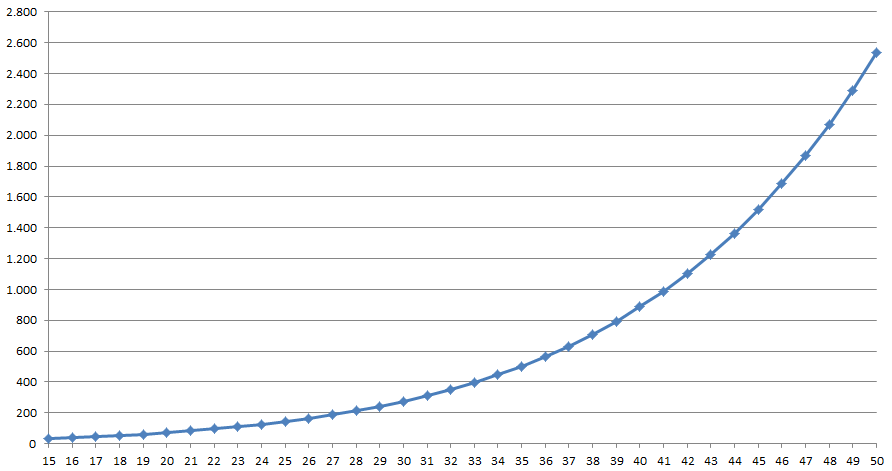
\includegraphics[scale=0.6]{stat_curves_theory.png}
\caption{The theoretical number of curves needed. For a $\beta$-bit factor
$e^{\sqrt{\frac{1}{2}\ln(2^\beta)\ln(\ln(2^\beta))}}$ is plotted. See remark \ref{rem:theory}.}
\label{fig:dedicatedAddition}
\end{figure}
\newline
\vfill
\begin{citat}{RSA message encoded in 1977 by Ron Rivest.}
The magic words are squeamish ossifrage\footnote{Rivest estimated that breaking this message by factoring the 125-digit number would require 40 quadrillion years. It was broken using idle times on machines connected to the internet.}.
\end{citat}